\subsection{Example: Slider-crank Mechanism}

\begin{frame}
	\begin{block}{Example 1: Slider-crank Mechanism}
		\begin{table}
			\begin{minipage}{0.5\linewidth}
				\begin{tabular}{l|l}
					      & $l_{AB}=l_1=0.5m$ \\
					Given & $l_{BC}=l_2=1m$ \\
					      & $\theta_1=60^\circ$ \\ \hline
					Find  & $x_C$ \\
				\end{tabular}
			\end{minipage}\hfill
			\begin{minipage}{0.5\linewidth}
				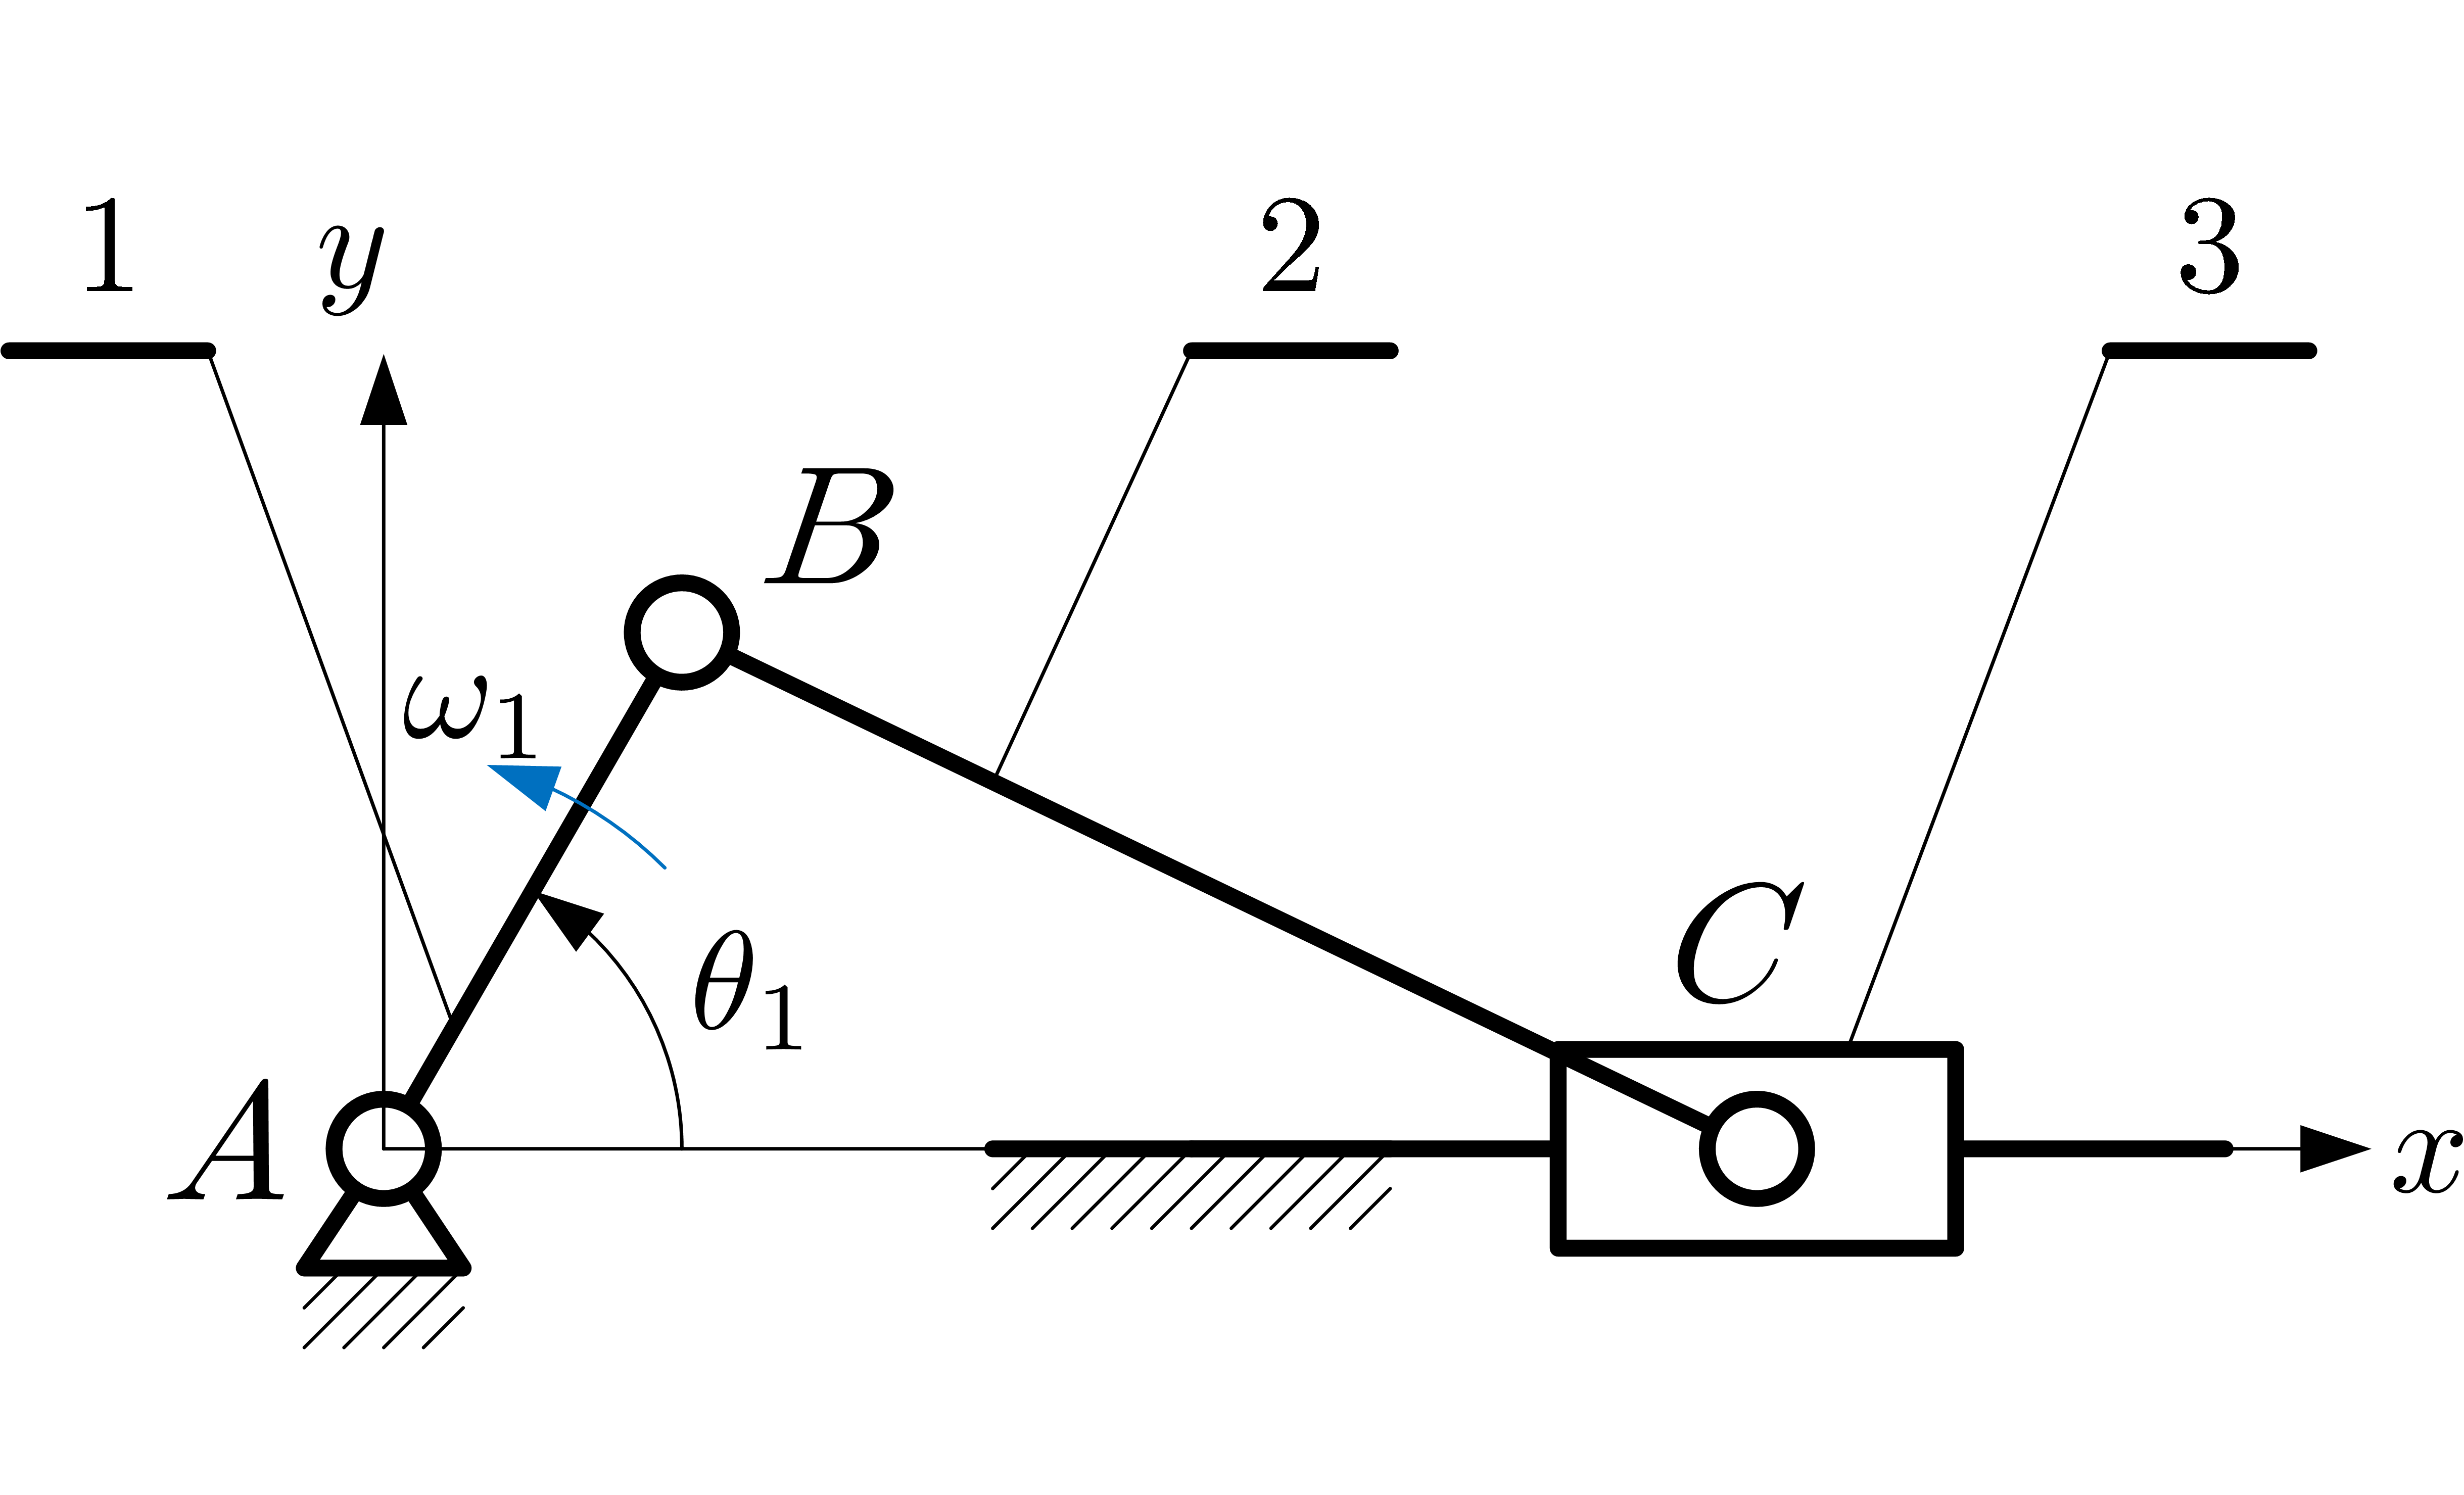
\includegraphics[width=50mm]{images/R-RRT.png}
			\end{minipage}
		\end{table}
	\end{block}
\emph{Solution 1}\vskip2.5mm
Position of joint $B$: $\displaystyle \vb{r}{B} = x_B\ih + y_B\jh = l_1\cos{\theta_1}\ih + l_1\sin{\theta_1}\jh$\\
Position of joint $C$: $\displaystyle \vb{r}{C} = x_C\ih$
\[
\Rightarrow(x_B-x_C)^2+y_B^2=l_1^2
\]
Solving the system of equations yields $x_{C_1}$ and $x_{C_2}$. Notice that in the mechanism, $x_C>x_B$ is the condition to obtain correct solution.
\end{frame}

\begin{frame}
\emph{Solution 2}\vskip2.5mm
Let $\vb{r}{B}=l_1\cos{\theta_1}\ih+l_1\sin{\theta_1}\jh$\vskip1.5mm
We can determine position of C by using direct solution:\vskip1.5mm
$\displaystyle\vb{r}{C}=\left(l_1\cos{\theta_1}+l_2\left(\arcsin{\frac{l_1\sin{\theta_1}}{l_2}}\right)\right)\ih$\vskip7.5mm
\emph{MATLAB R2019a code}\\
\lstinputlisting[style=Matlab-editor, basicstyle=\mlttfamily]{codes/RRRT-position2.m}
\end{frame}


\begin{frame}{MATLAB R2019a code}
	\lstinputlisting[style=Matlab-editor, basicstyle=\mlttfamily]{codes/RRRT-position1.m}
\end{frame}
\begin{frame}{Plotting using MATLAB R2019a}
	\lstinputlisting[style=Matlab-editor, basicstyle=\mlttfamily]{codes/RRRT-plot.m}
\end{frame}
\begin{frame}{Output figure}
\centering
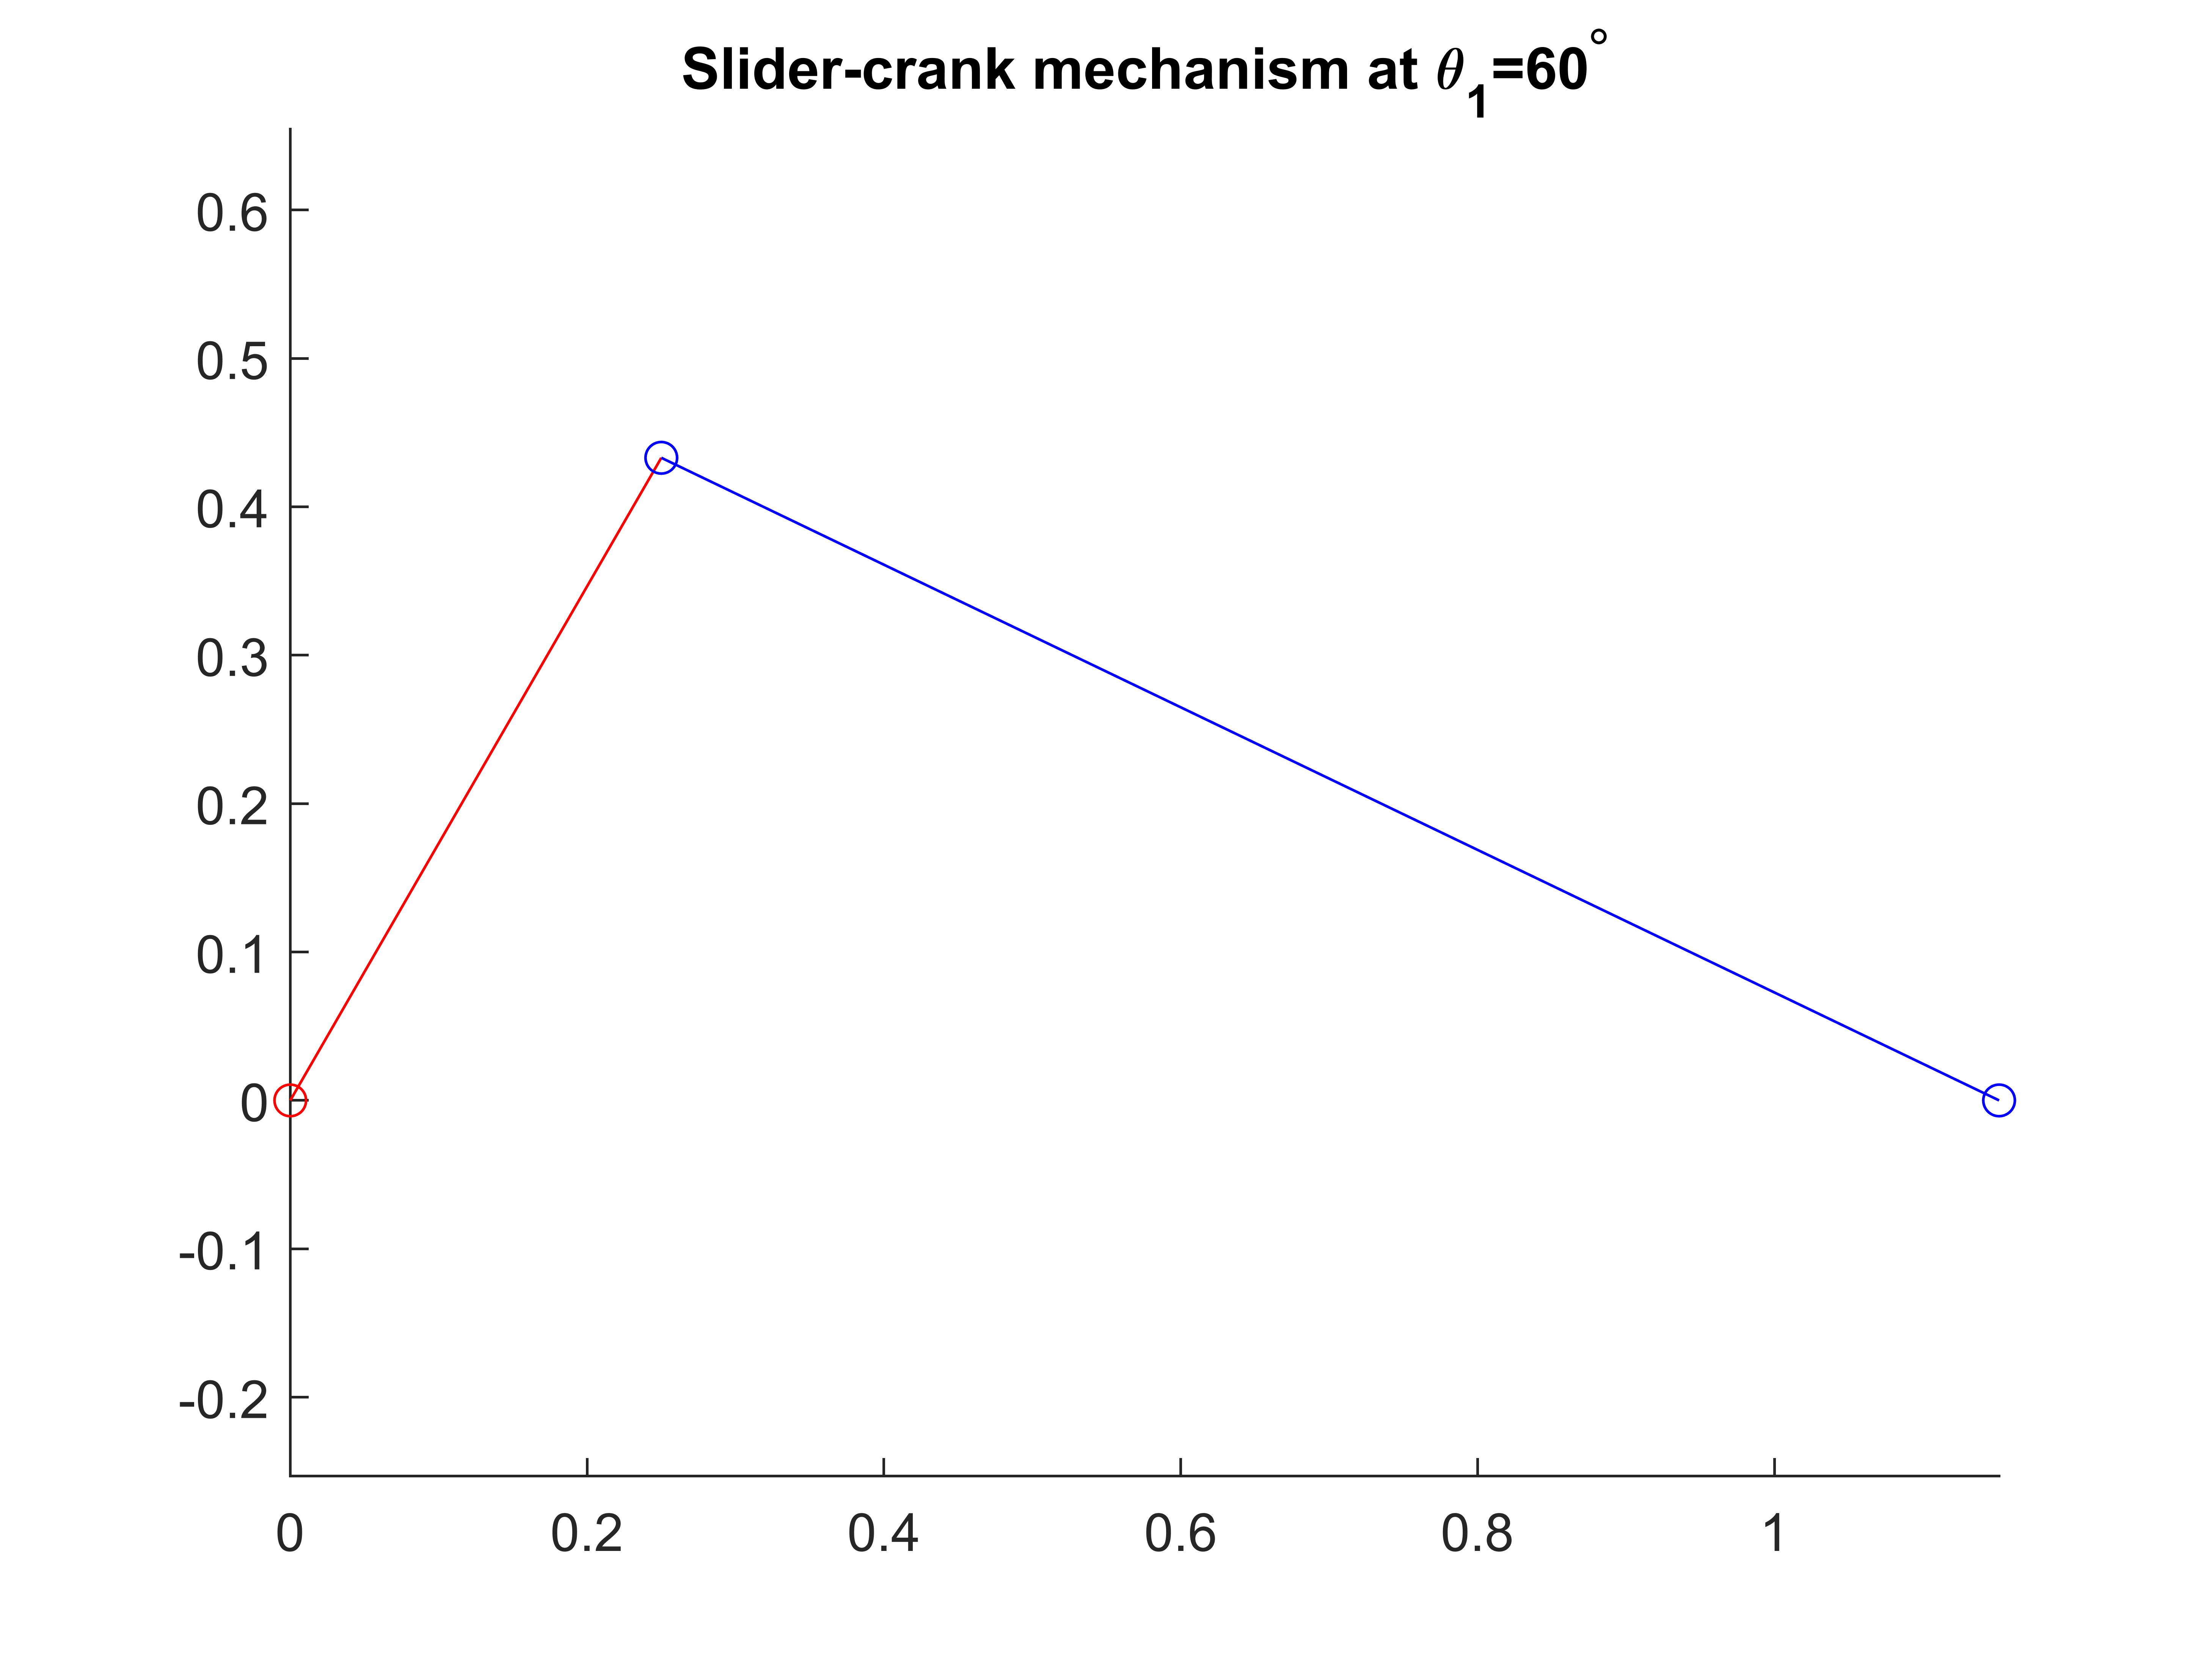
\includegraphics[width=100mm]{images/RRRT-plot.png}
\end{frame}
\begin{frame}{Trajectory plotting using MATLAB R2019a}
\lstinputlisting[style=Matlab-editor, basicstyle=\mlttfamily]{codes/RRRT-trajectory.m}
\end{frame}
\begin{frame}{Output figure}
\centering
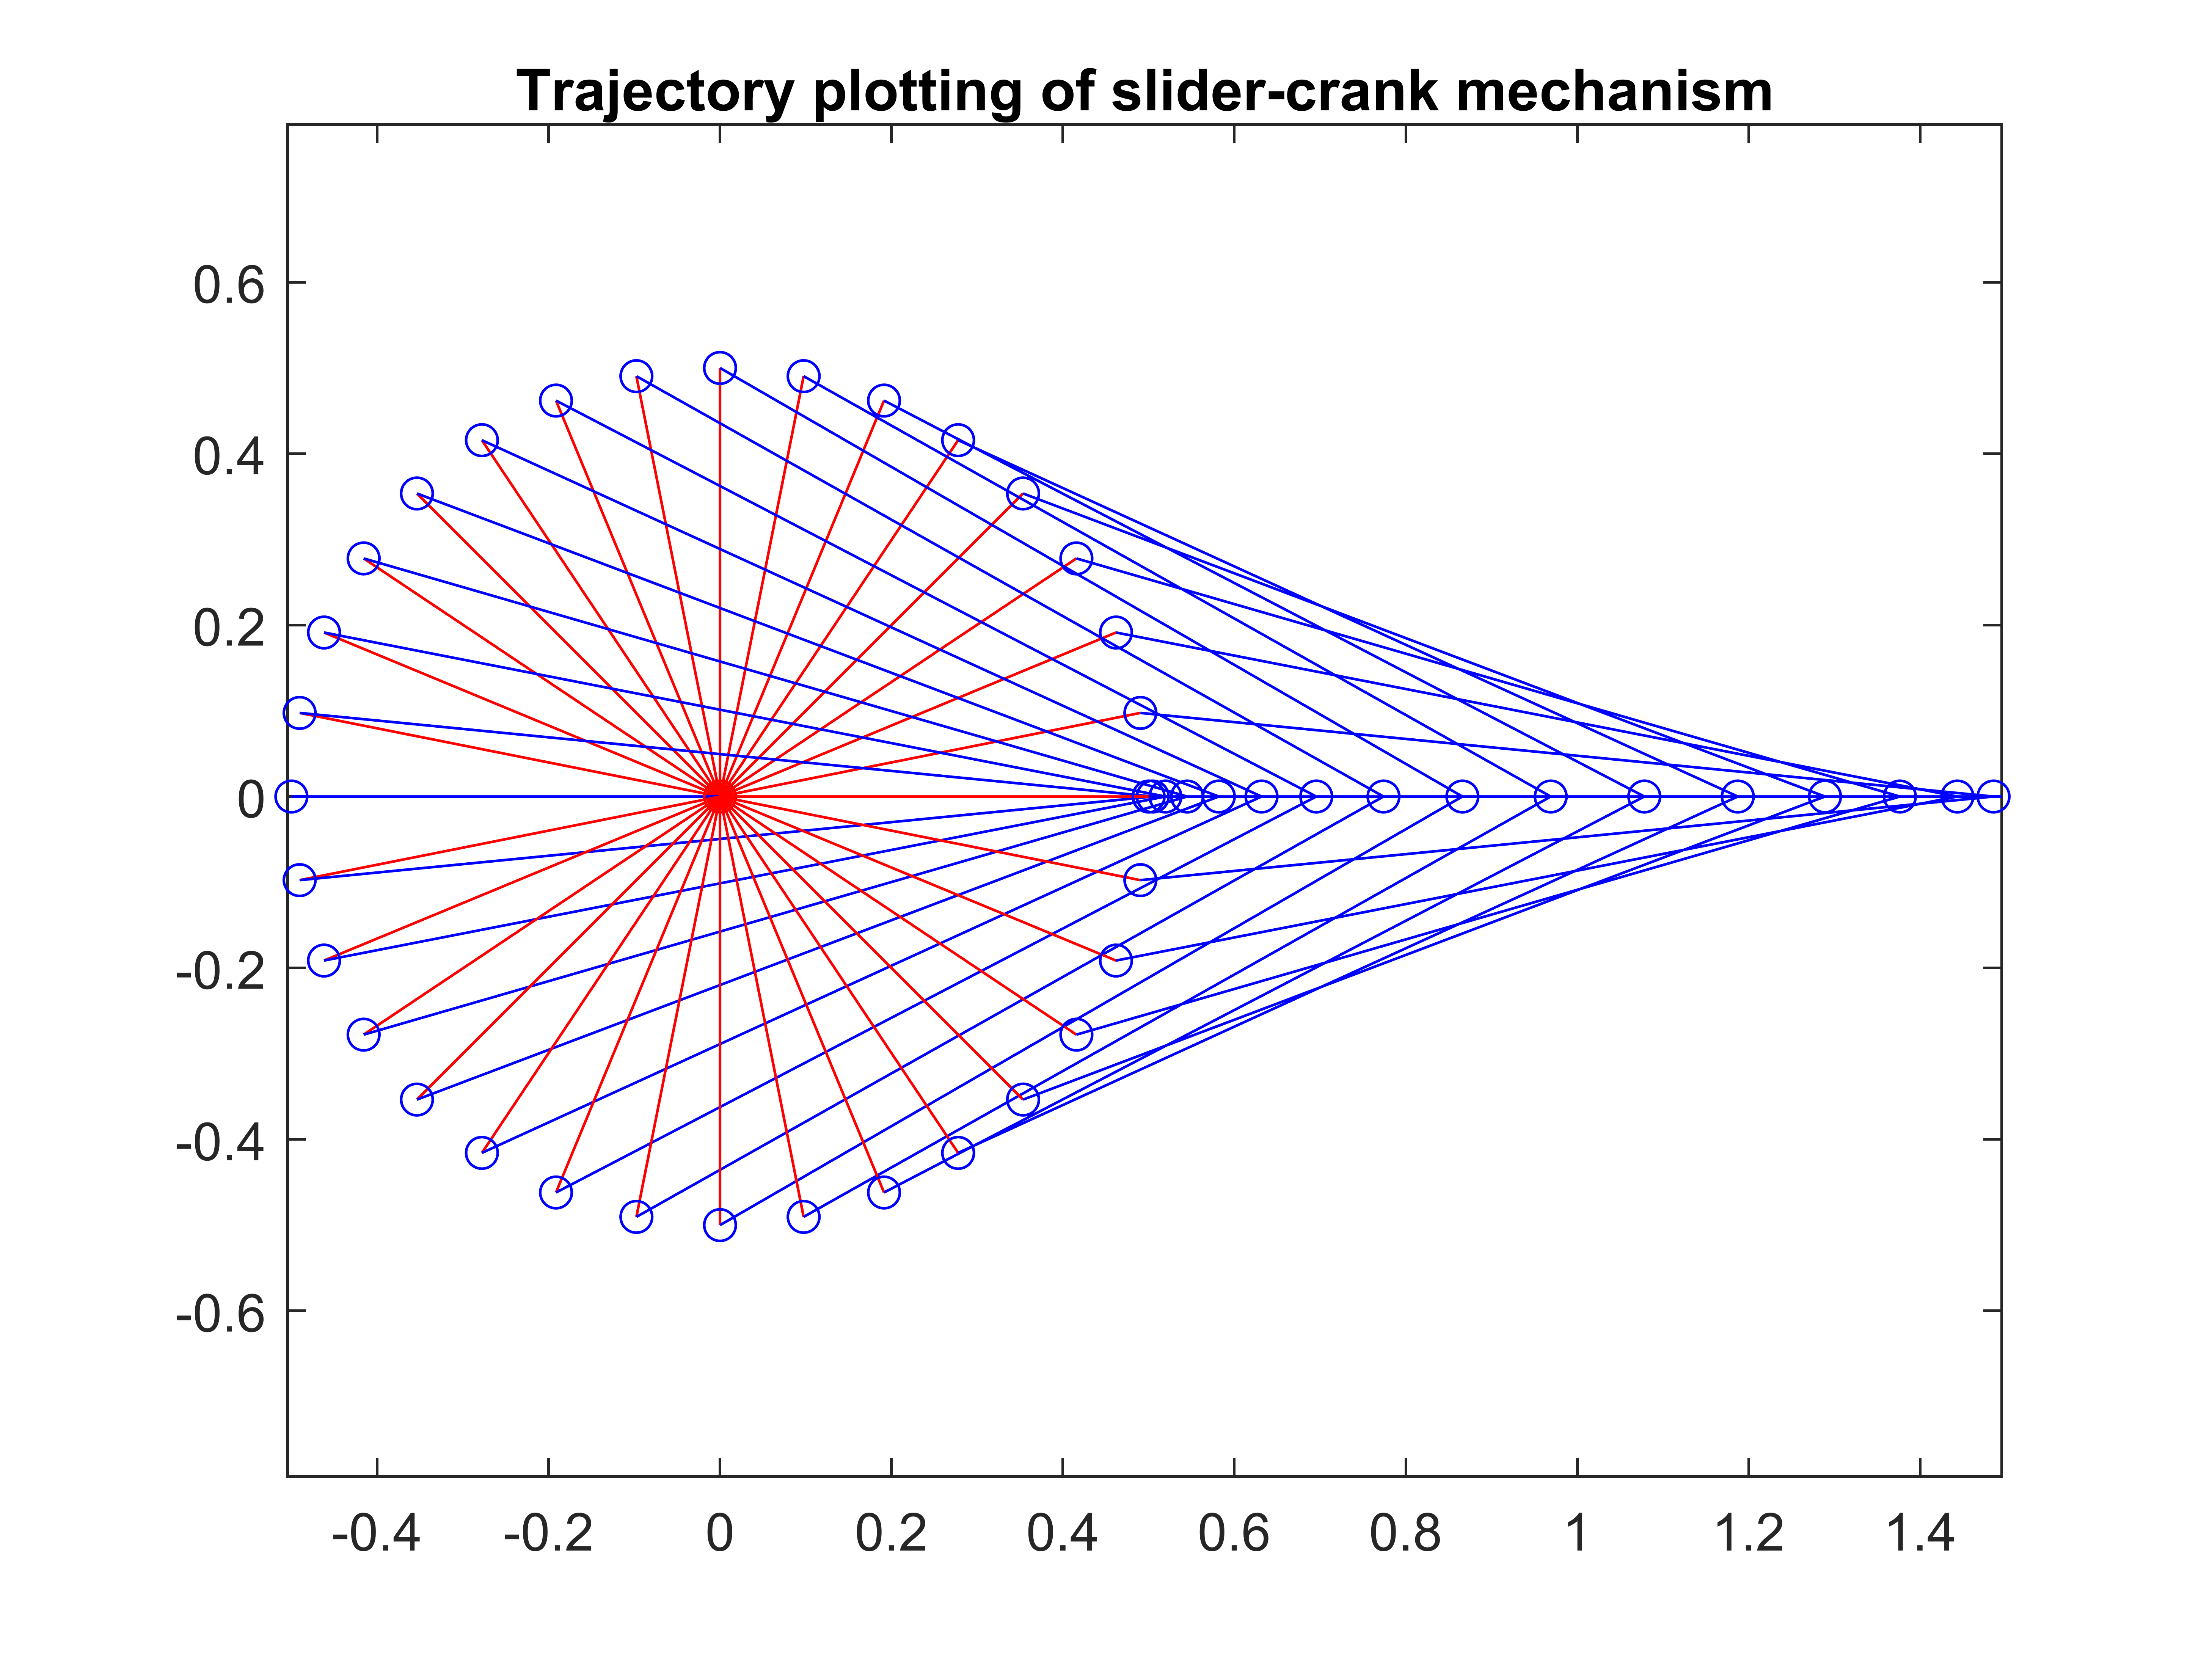
\includegraphics[width=100mm]{images/RRRT-trajectory.png}
\end{frame}